\newpage
\section{Zakończenie}
\label{sec:zakonczenie}

\subsection*{Podsumowanie realizacji celu pracy}

Celem pracy, sformułowanym w~rozdz.~\ref{sec:wstep}, było zaprojektowanie i~implementacja systemu
monitorowania położenia zwierząt w~czasie rzeczywistym, działającego w~obszarach pozbawionych
pokrycia sieci komórkowej, wraz z~aplikacją mobilną umożliwiającą wizualizację położenia na mapie,
definiowanie wirtualnych stref bezpieczeństwa oraz powiadamianie użytkownika o~ich przekroczeniu.

Cel ten został zrealizowany. Rozdz.~\ref{sec:wymagania} przełożył motywację (ucieczki psa myśliwskiego
poza teren pozbawiony ogrodzenia i~zasięgu sieci komórkowej) na trzy konkretne problemy inżynierskie -
transmisję danych bez infrastruktury zewnętrznej, optymalizację zajętości pasma oraz integrację
aplikacji mobilnej z~siecią radiową - a~także na mierzalne wymagania funkcjonalne i~parametryczne.
Rozdz.~\ref{sec:modulacja-lora} opisuje dobór technologii LoRa/Meshtastic i~konfigurację sprzętu
radiowego rozwiązujący problem pierwszy, rozdz.~\ref{sec:integracja-meshtastic} - integrację aplikacji
mobilnej z~siecią radiową (problem trzeci), a~rozdz.~\ref{sec:geofencing} - mechanizm geofencingu
oparty na algorytmie ray casting wraz z~modelem stref i~zdarzeń. Rozdz.~\ref{sec:podsumowanie-testy}
potwierdza w~oparciu o~testy terenowe, że zbudowany system poprawnie wykrywa przekroczenie granicy
strefy zarówno w~typowych, jak i~skrajnych warunkach.

Problem drugi - optymalizacja zajętości pasma poprzez adaptacyjną częstotliwość wysyłania pozycji
zależną od stanu ruchu węzła - pozostaje częściowo otwarty; w~przeprowadzonych testach system
korzystał ze stałego interwału próbkowania GPS (5~s) narzuconego przez firmware Meshtastic
(por.\ rozdz.~\ref{sec:podsumowanie-testy}), a~nie z~mechanizmu adaptacyjnego. Kwestię tę rozwinięto
w~rozdziale ,,Możliwości dalszego rozwoju''.

\subsection*{Wnioski z~oceny rozwiązania}

Zestawienie z~komercyjnymi systemami śledzenia psów myśliwskich (tab.~\ref{tab:porownanie}) oraz
wyniki testów terenowych (rozdz.~\ref{sec:podsumowanie-testy}) pozwalają sformułować następujące
wnioski.

Architektura mesh nie ogranicza zasięgu systemu do pojedynczego łącza
nadajnik-odbiornik, jak w~rozwiązaniach Dogtra i~Dogtrace, lecz pozwala go rozszerzać przez
dodawanie kolejnych węzłów pośredniczących - potwierdzają to testy zasięgu
(tab.~\ref{tab:zasieg-efektywny}), w~których dodanie trzeciego węzła zwiększyło zasięg efektywny
z~2052~m do 2278~m. System zbudowany jest z~ogólnodostępnych komponentów za ok.\ 400~PLN za węzeł,
czyli znacząco taniej niż rozwiązania komercyjne (2500~PLN i~2300~PLN), przy jednoczesnym braku
sztywnego limitu liczby węzłów (21 dla Dogtra, 19 dla Dogtrace). Testy precyzji geofencingu
(rozdz.~\ref{sec:precyzja-geofencingu}) wykazały, że wprowadzenie bufora rzędu 6-8~m redukuje
liczbę fałszywych alarmów o~99,6\%, co czyni system praktycznie użytecznym mimo ograniczeń
interwału próbkowania GPS.

Niestety system ma też swoje ogranicznia. Osiągnięty zasięg efektywny (889-2278~m, zależnie od konfiguracji
sprzętowej) jest o~rząd wielkości mniejszy niż w~systemach komercyjnych (14-20~km) - należy jednak
podkreślić, że są to wartości nieporównywalne wprost, ponieważ zasięg systemu mesh rośnie wraz
z~liczbą węzłów pośredniczących, a~zasięg systemów punkt-punkt jest stały. Dodatkowo deklarowane przez producentów
marketingowe metryki często nie w znacznej mierze nie pokrywają się z rzeczywistymi wartościami. Co istotne, konfiguracja
bazowa oparta wyłącznie na węzłach T-1000-E (889~m) \emph{nie spełnia} przyjętego w~rozdz.~\ref{sec:wymagania}
wymagania minimalnego zasięgu 2~km - wymaganie to jest spełnione dopiero po zastosowaniu węzła
T-Beam po stronie bazy (2052~m) lub dodaniu przekaźnika (2278~m). Błąd zgłoszenia przekroczenia
granicy strefy jest w~praktyce zdominowany przez interwał próbkowania GPS (5~s), a~nie przez
niedoskonałości algorytmu ray casting - jest to ograniczenie po stornie sprzętu i protokołu (firmware
Meshtastic), a~nie implementacyjne. Jako ostatnie ogranicznie trzeba zwrócić uwagę na to, że ochrona 
obudowy węzła mobilnego (IP65) jest niższa niż w~rozwiązaniach komercyjnych (IPX9K, IP68).

\subsection*{Zakres zastosowań i~perspektywy wdrożenia}

Choć bezpośrednim punktem wyjścia było śledzenie psa myśliwskiego, opracowane rozwiązanie -
sieć mesh LoRa z~aplikacją mobilną obsługującą geofencing dowolnych wielokątów - nie jest
specyficzne dla tego jednego zastosowania. Ten sam mechanizm mógłby posłużyć do monitorowania
zwierząt gospodarskich na dużych, otwartych pastwiskach pozbawionych zasięgu sieci komórkowej,
innych zwierząt domowych, a~także - po odpowiednich modyfikacjach interfejsu - do pilnowania mienia
lub sprzętu pozostawionego w~terenie (analogicznie do funkcji WAYPOINT/FENCE oferowanych przez
Dogtrace, tab.~\ref{tab:porownanie}).

Przed wdrożeniem produkcyjnym system wymagałby jednak dodatkowej walidacji, wykraczającej poza
zakres niniejszej pracy:
\begin{itemize}
    \item pomiaru rzeczywistego czasu pracy węzła mobilnego na baterii w~warunkach terenowych
          (aspekt ten nie był przedmiotem testów opisanych w~rozdz.~\ref{sec:podsumowanie-testy}),
    \item testów z~większą liczbą jednocześnie monitorowanych zwierząt/węzłów niż trzy użyte
          w~testach zasięgu,
    \item potwierdzenia szczelności obudowy w~warunkach długotrwałej ekspozycji (deszcz, błoto,
          zanurzenie częściowe) wykraczających poza deklarację IP65,
    \item oszacowania kosztu produkcji seryjnej (obecna wycena ok.\ 400~PLN/węzeł dotyczy
          pojedynczych egzemplarzy, por.\ tab.~\ref{tab:porownanie}).
\end{itemize}

\newpage
\subsection*{Możliwości dalszego rozwoju}

Na podstawie zidentyfikowanych ograniczeń można wskazać kilka kierunków dalszego rozwoju systemu.
Szczególnie istotne wydaje się zrealizowanie adaptacyjnej częstotliwości wysyłania pozycji,
zależnej od stanu ruchu węzła - a więc rzadszego próbkowania podczas bezruchu i~częstszego
w~pobliżu granicy strefy - co pozwoliłoby wypełnić wymaganie sformułowane w~rozdz.~\ref{sec:wymagania},
dotychczas niezrealizowane wobec stałego interwału próbkowania GPS narzuconego przez firmware
Meshtastic. Poza oczywistą korzyścią w~postaci oszczędności baterii węzła mobilnego, rozwiązanie
to miałoby również bezpośredni wpływ na jakość działania systemu: skrócenie efektywnego interwału
próbkowania w~otoczeniu granicy strefy powinno zmniejszyć błąd zgłoszenia przekroczenia opisany
w~rozdz.~\ref{sec:precyzja-geofencingu}, bez konieczności utrzymywania wysokiej częstotliwości
próbkowania - a~więc i~zwiększonego zużycia energii oraz pasma - na całym obszarze monitorowanym.
Kolejnym kierunkiem wartym zbadania jest współpraca z~dronem, wykorzystanym w~niniejszej
pracy dotychczas jedynie jako narzędzie testowe do odtwarzania powtarzalnej trasy węzła mobilnego.
Docelowo dron mógłby pełnić funkcję aktywnego elementu systemu - unoszący się nad terenem węzeł, 
dzięki wyniesieniu ponad przeszkody terenowe, mógłby zwiększać zasięg poszukiwań zagubionego 
zwierzęcia oraz poprawiać parametry transmisji (mniejsze tłumienie sygnału, większą niezawodność łącza)
względem konfiguracji opartej wyłącznie na stacjonarnej lub noszonej stacji bazowej.

Dodatkowych badań wymagałyby również testy skalowalności sieci przy liczbie węzłów większej niż
trzy, w~tym analiza zajętości współdzielonego kanału radiowego, sygnalizowana już w~tab.~\ref{tab:porownanie}
(przypis dotyczący nieograniczonej liczby węzłów), a~także pomiar i~optymalizacja czasu pracy na
baterii węzła mobilnego wraz z~doborem trybów oszczędzania energii w~zależności od aktywności
zwierzęcia. Możliwe byłoby wreszcie rozszerzenie aplikacji mobilnej o~analitykę historycznych tras,
wykraczającą poza obecny eksport CSV opisany w~rozdz.~\ref{sec:historia-eksport}, oraz o~wersję
na system iOS.

Z powyższych kierunków szerzej przyjrzymy się pierwszemu, ponieważ miałby on realnie największy wpływ na użytkowanie.
Jak wynika z otwartego kodu firmware'u Meshtastic~\cite{meshtasticFirmwareRepo} oraz opisu API
modułów~\cite{meshtasticModuleApiDocs}, częstotliwością raportowania pozycji sterują dwa oddzielne ustawienia. Jedno ustala, jak często moduł GPS
w~ogóle próbuje złapać nowy namiar, a drugie jak często węzeł nadaje posiadaną pozycję do sieci.
Domyślnie są to odpowiednio 2~minuty i~godzina - w~tej pracy oba skrócono do 5~s, żeby uzyskać
,,gęstszy'' strumień pozycji.

Firmware ma też wbudowany, domyślnie włączony mechanizm ,,inteligentnego'' raportowania: węzeł
nadaje pozycję od razu, gdy przesunie się o~więcej niż jakieś 100~metrów, zamiast czekać na koniec
stałego interwału. To dokładnie ten rodzaj mechanizmu - reagującego na ruch węzła, a~nie na zegar -
był potrzebny do pełnej realizacji ,,problemu drugiego''. Z~kodu wynika jednak, że odstęp między
takimi nadaniami i~tak nie może zejść poniżej 5~minut, niezależnie od tego, co ustawi użytkownik -
to twardy limit wpisany w~firmware. W~praktyce ten wbudowany mechanizm okazuje się więc wolniejszy
niż zwykły, stały interwał 5-sekundowy zastosowany w~pracy i~sam z~siebie nie rozwiązuje problemu
opóźnienia poniżej 3~sekund.

Dosłowne spełnienie tego wymagania wymagałoby więc czegoś więcej niż zmiany ustawień. Jedną
z~opcji byłoby dynamiczne przeprogramowywanie interwału z~poziomu aplikacji mobilnej - skoro
aplikacja już zna geometrię stref i~bieżącą pozycję węzła, mogłaby skracać interwał raportowania
tylko wtedy, gdy zwierzę zbliża się do granicy, a~rozluźniać go w~pozostałym czasie dla
oszczędności baterii. Głębszym, ale trwalszym rozwiązaniem byłoby napisanie własnego modułu 
firmware'u, który przenosiłby geometrię stref na sam węzeł i~decydował o~częstotliwości nadawania
lokalnie, bez pośrednictwa telefonu. Odbyłoby się to kosztem konieczności utrzymywania własnego forka firmware'u.

    Testy zasięgu przebiegały etapami, w~bardzo różnych warunkach terenowych, zanim ostatecznie
oceniono system w~scenerii zbliżonej do docelowego zastosowania. Pierwsze pomiary wykonano
w~zabudowie wielopiętrowej mieszkalnej (widocznej w~tle części zrzutów ekranu w~rozdz.
,,Przegląd ekranów aplikacji'', np.\ rysunek~\ref{fig:map-screen})
i~wykazały zasięg praktycznie ograniczony do bezpośredniej widoczności między węzłami. Kolejne
testy, przeprowadzone na płaskim, otwartym terenie polnym, dały wynik rzędu 2~km, a~testy
w~terenie górskim - rzędu 10~km. Dla porównania, oficjalne testy zasięgu Meshtastic~\cite{meshtasticRangeTests} dokumentują przypadki nawiązania
łączności na dystansie sięgającym kilkuset kilometrów - trzeba jednak wyraźnie zastrzec, że są to
warunki skrajnie sprzyjające (bezpośrednia widzialność optyczna, znaczna wysokość umieszczenia
anten, sprzyjająca propagacja radiowa), zupełnie niereprezentatywne dla docelowego zastosowania
systemu, czyli obroży psa poruszającego się nisko nad ziemią, w~terenie często zalesionym.

Dopiero testy przeprowadzone w~scenerii najbliższej docelowej tnz. terenie o charakterze rolniczo-leśnym na
Mazurach- pokazały, że efektywny zasięg gwarantujący dostarczenie 90\% pakietów jest znacząco mniejszy niż sugerowałyby wcześniejsze pomiary w~terenie
otwartym czy górskim (889-2278~m, tab.~\ref{tab:zasieg-efektywny}). Zależność zasięgu systemu od
typu terenu okazała się na tyle silna, że wynik uzyskany w~jednych warunkach nie przekładał się
wprost na inne - nie był to wniosek oczywisty na początku realizacji pracy.

Gdybym zaczynał pracę od nowa, zakupiłbym bardziej różnorodny zbiór modułów Meshtastic, o różnych parametrach anten oraz baterii, aby przetestować
różne kombinacje sprzętu w~roli stacji bazowej jeszcze przed ostatecznym wyborem platformy
(rozdz.~\ref{sec:modulacja-lora}), zamiast dopiero w~testach końcowych
(rozdz.~\ref{sec:zasieg-siec}). Pozwoliłoby to ocenić zależność zasięgu od typu anteny i~mocy
nadajnika na wczesnym etapie projektu i~ewentualnie skorygować dobór sprzętu, zanim wybór ten
wpłynął na architekturę całego systemu. 
\newpage
Na zakończenie pracy przedstawiam, często wspominanego w tej pracy, psa rasy Mały Gończy Gaskoński, który był inspiracją dla stworzenia niniejszej pracy oraz
służył do testów w terenie. 

\begin{figure}[!t]
  \centering
    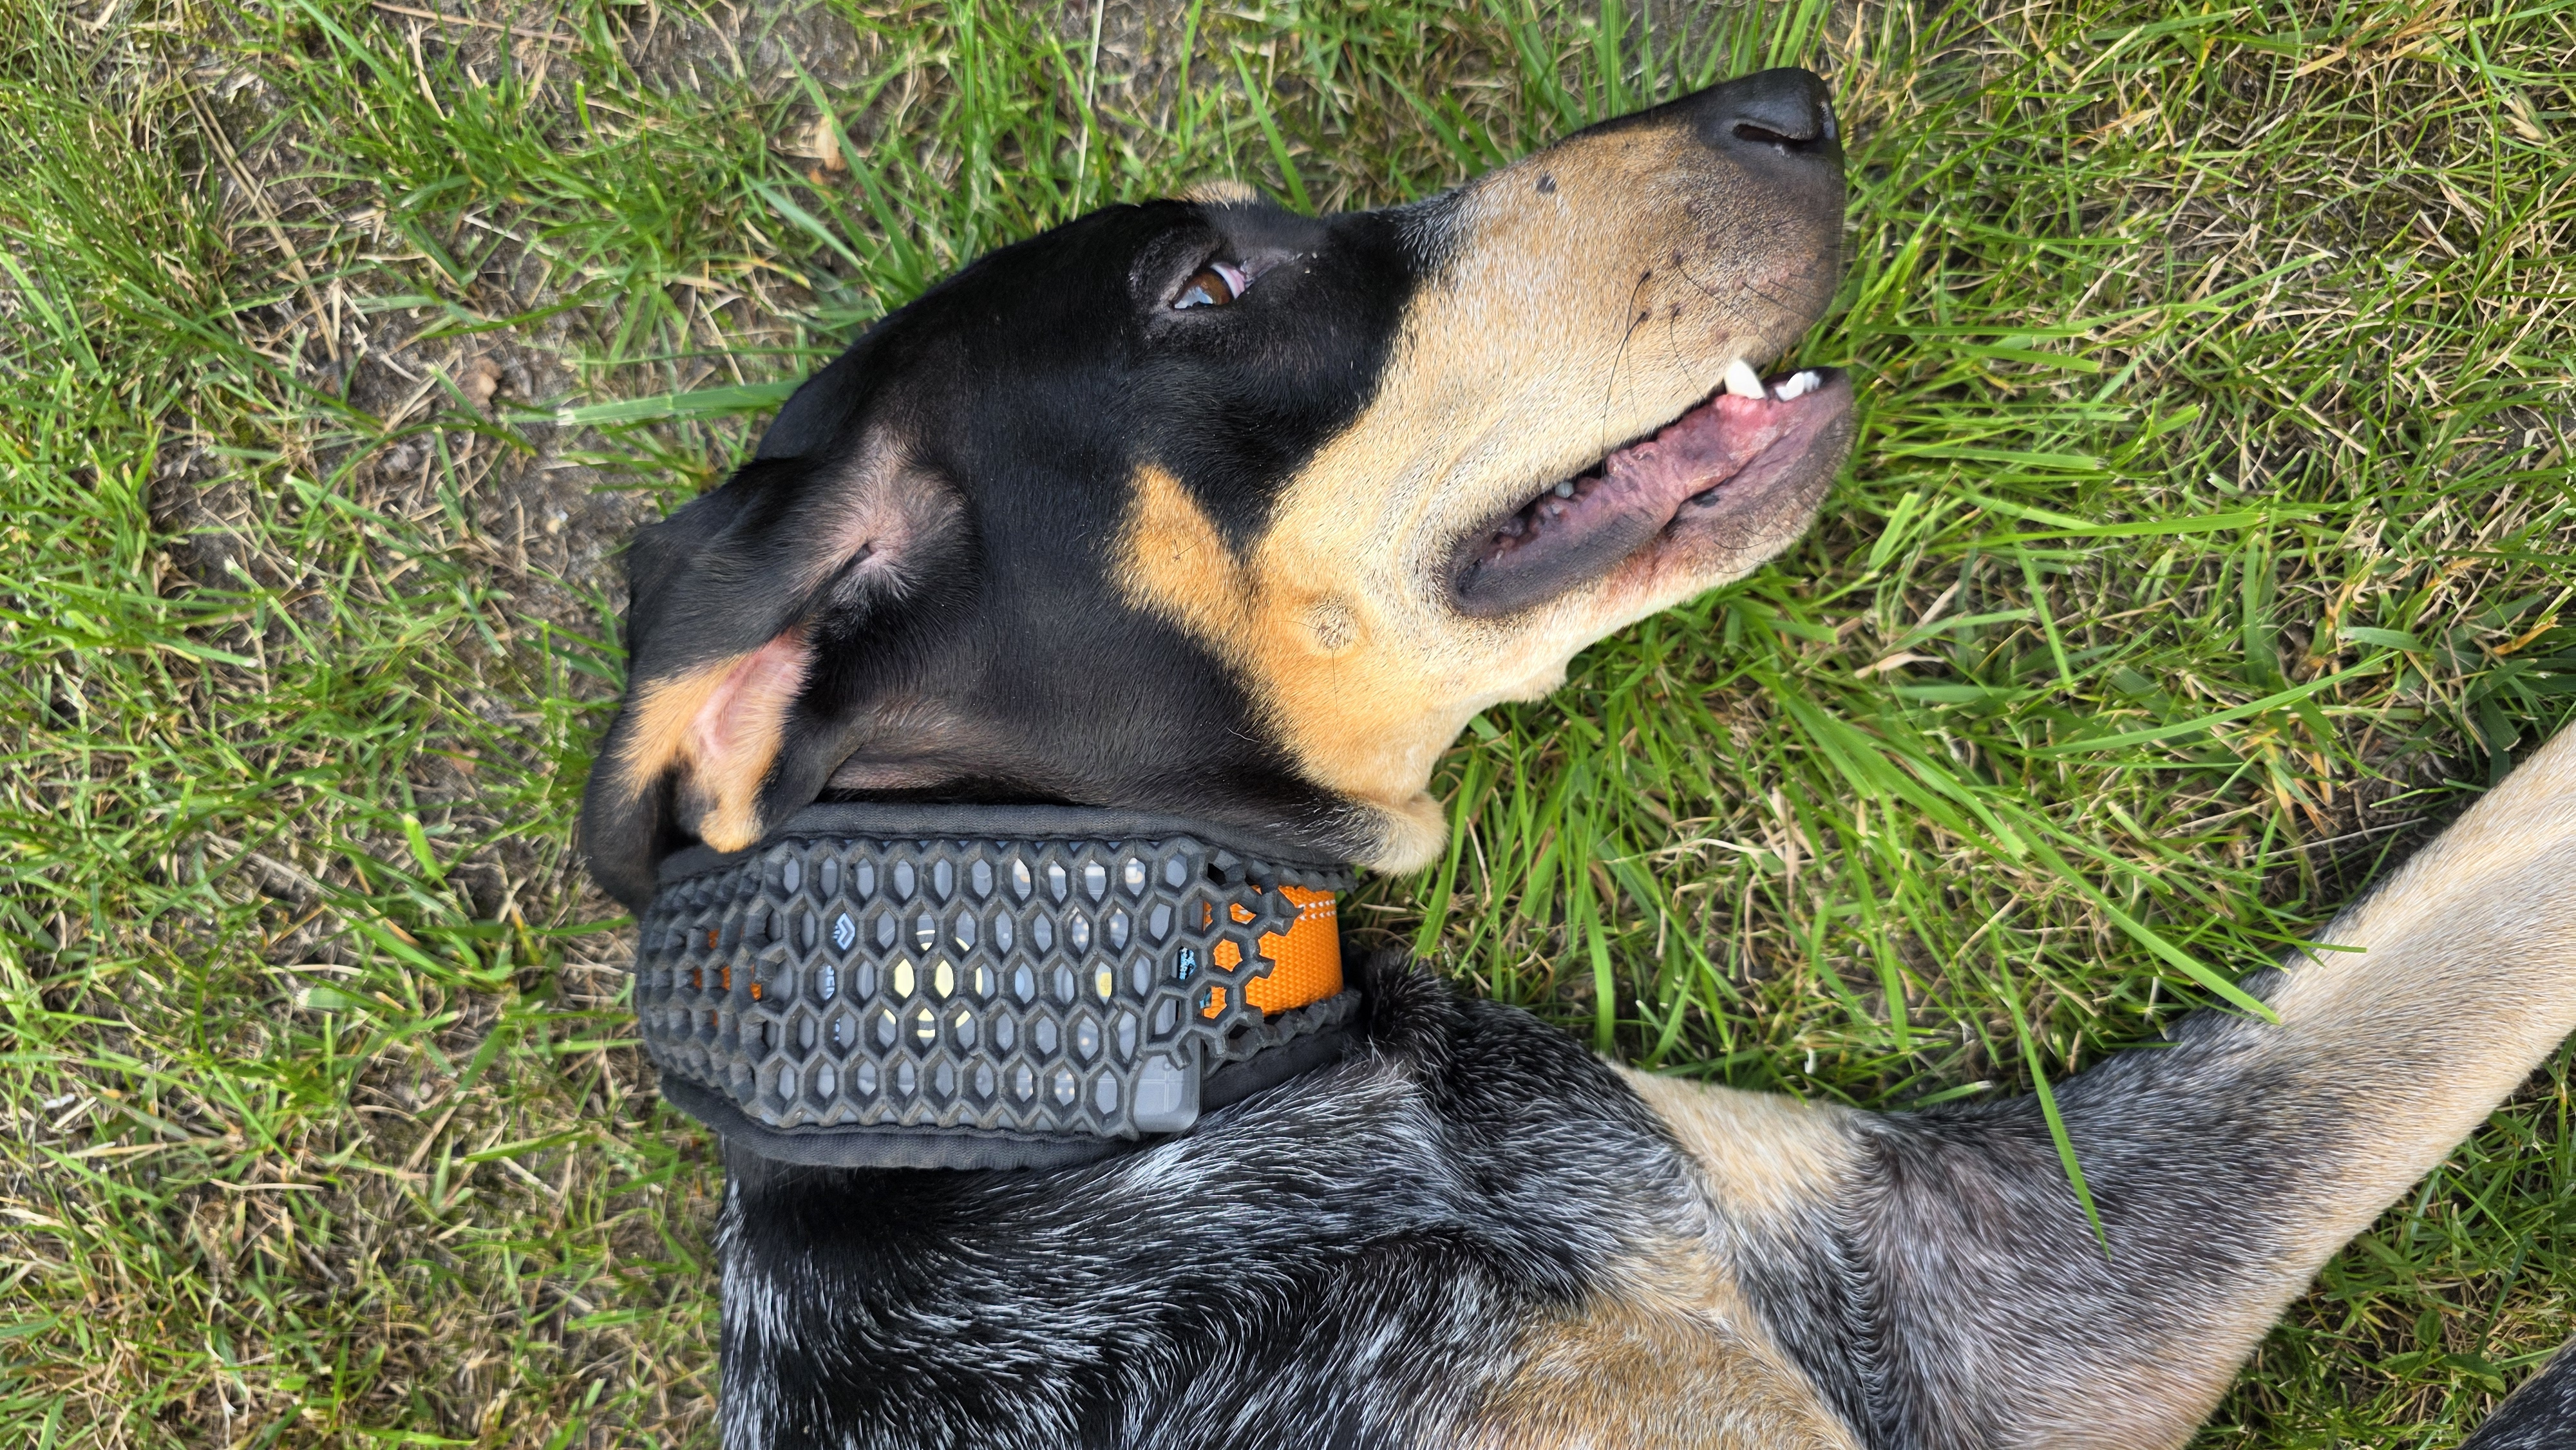
\includegraphics[width=0.8\linewidth]{WUT-Thesis/img/reja_meshtracker.jpg}
    \caption{Mały gończy Gaskoński}
    \label{fig:piesDoTestow}
\end{figure}